% Created 2020-02-21 Fri 13:43
% Intended LaTeX compiler: pdflatex
\documentclass[presentation]{beamer}
\usepackage[utf8]{inputenc}
\usepackage[T1]{fontenc}
\usepackage{graphicx}
\usepackage{grffile}
\usepackage{longtable}
\usepackage{wrapfig}
\usepackage{rotating}
\usepackage[normalem]{ulem}
\usepackage{amsmath}
\usepackage{textcomp}
\usepackage{amssymb}
\usepackage{capt-of}
\usepackage{hyperref}
\usetheme{metropolis}
\usecolortheme{}
\usefonttheme{}
\useinnertheme{}
\useoutertheme{}
\author{Petru Rebeja, Marius Apetrii}
\date{20 Februarie 2020}
\title{Tehnici Avansate de Programare}
\subtitle{Infrastructură și unelte}
\institute[UAIC]{Facultatea de Matematică\\Universitatea Alexandru Ioan Cuza, Iași}
\hypersetup{
 pdfauthor={Petru Rebeja, Marius Apetrii},
 pdftitle={Tehnici Avansate de Programare},
 pdfkeywords={},
 pdfsubject={},
 pdfcreator={Emacs 26.3 (Org mode 9.3.6)},
 pdflang={Romanian}}
\begin{document}

\maketitle
\begin{frame}[label={sec:orgc1b01dd}]{Informații}
Pagina cursului: \url{https://rebeja.eu/dotnet-math}

\begin{center}

\includegraphics[height=0.6\textheight]{img/qr-pagina-curs.png}
\end{center}
\end{frame}
\begin{frame}[label={sec:orgafb33b9}]{Ciclul de dezvoltare al aplicațiilor}
\begin{center}
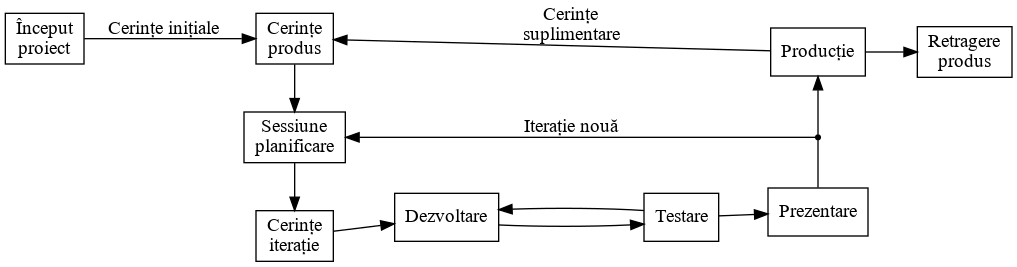
\includegraphics[width=\textwidth]{./img/ciclul-agile.png}
\end{center}
\end{frame}
\begin{frame}[label={sec:org68989d3}]{Etapa I: Identificarea unei nevoi}
Un sistem software trebuie să satisfacă o anumită nevoie a utilizatorului:
\begin{itemize}
\item Automatizarea procesului manual,
\item Performanță sporită
\item Etc.
\end{itemize}
\end{frame}
\begin{frame}[label={sec:orge71840f}]{Etapa II: Cerințe inițiale}
\begin{itemize}
\item După identificarea nevoii se alcătuiește lista de cerințe inițiale.
\item Opțional, se identifică atributele arhitecturale suplimentare ale sistemului.
\end{itemize}
\end{frame}
\begin{frame}[label={sec:org48333a3}]{Etapa III: Minimum Viable Product}
Din lista cerințelor inițiale se aleg cele care constituie un minim de viabilitate pentru proiect.
\begin{definition}[Minimum viable product]
Versiune a produsului software care conține o cantitate suficientă de funcționalitate pentru a satisface utilizatorii timpurii.\footnote{\url{https://en.wikipedia.org/wiki/Minimum\_viable\_product}}
\end{definition}
\end{frame}
\begin{frame}[label={sec:org7f32178}]{Etapa IV: Dezvoltarea în iterații}
\begin{itemize}
\item Cerințele sunt ordonate în funcție de importanță.
\item Echipa alege \(N\) cele mai importante cerințe.
\end{itemize}
\end{frame}
\begin{frame}[label={sec:org54a4613}]{Etapa IV: Dezvoltarea în iterații (cont.)}
\begin{itemize}
\item Mai întâi se planifică abordarea (task breakdown).
\item Fiecare membru ia câte o sarcină.
\end{itemize}
\end{frame}
\begin{frame}[label={sec:org9f6cb43}]{Etapa IV: Dezvoltarea în iterații (cont.)}
\begin{itemize}
\item Când o funcționalitate este gata, ea trece la testare.
\item Dacă este conformă cu cerințele, aceasta este marcată ca finalizată.
\item Altfel, revine la programator.
\end{itemize}
\end{frame}
\begin{frame}[label={sec:orge85be7d}]{Etapa IV: Dezvoltarea în iterații (cont.)}
\begin{itemize}
\item La sfârșitul iterației se face o prezentare a funcționalităților implementate.
\item Procesul se reia într-o iterație nouă.
\end{itemize}
\end{frame}
\begin{frame}[label={sec:org66a4ce7}]{Etapa V: Lansarea în producție}
\begin{itemize}
\item Lansarea în producție se face când:
\begin{itemize}
\item Avem suficientă funcționalitate implementată.
\item Situația o impune (urgențe, defecte etc.).
\end{itemize}
\end{itemize}
\end{frame}
\begin{frame}[label={sec:orgcf7f9af}]{Etapa VI: Întreținerea și dezvoltarea}
\begin{itemize}
\item Utilizatorii semnalează erori și cer funcționalități noi.
\item Acestea sunt adăugate la lista de cerințe.
\end{itemize}
\end{frame}
\begin{frame}[label={sec:orgfd220c5}]{Etapa VII: Retragerea produsului}
Se întâmplă din mai multe motive:
\begin{itemize}
\item Nu aduce încasări suficiente,
\item Perimare
\item Etc.
\end{itemize}
\end{frame}
\begin{frame}[label={sec:org89c4194}]{Unelte pentru dezvoltare}
\begin{center}

\includegraphics[width=.9\linewidth]{img/vs2019.jpg}
\end{center}
Imagine preluată \footnote{\url{https://dev.infohub.cc/wp-content/uploads/2019/04/vs2019.jpg}}
\end{frame}
\begin{frame}[label={sec:org646cdb9}]{Bune practici în scrierea codului-sursă}
\begin{itemize}
\item Codul-sursă trebuie scris în limba engleză.
\item Textul trebuie să fie preluat dintr-un set de resurse.
\item Alegeți tipul de date potrivit.
\item Rescrieți codul, nu dați copy/paste.
\item Dacă nu există în sistemul de păstrare a istoricului atunci nu există.
\end{itemize}
\end{frame}
\begin{frame}[label={sec:orga549027}]{Păstrarea istoricului codului-sursă}
\begin{itemize}
\item Produsele software mari pot ajunge și la milioane de linii de cod.
\item Sistemele de control al reviziilor (version control systems) ne permit:
\begin{itemize}
\item Să vedem toate modificările făcute asupra unui fișier,
\item Să revenim la o versiune anterioară,
\item Să lucrăm mai multe persoane simultan la același fișier.
\end{itemize}
\end{itemize}
\end{frame}
\begin{frame}[label={sec:org80879bb}]{Git}
\begin{block}{Git SCM}
Git este un sistem de control al reviziilor open-source, distribuit și gratuit. Sistemul a fost proiectat să gestioneze rapid și eficient proiecte de toate dimensiunile.\footnote{\url{https://git-scm.com/}}
\end{block}
\end{frame}
\begin{frame}[label={sec:orgf863c23}]{Fluxul de lucru Git}
\begin{center}
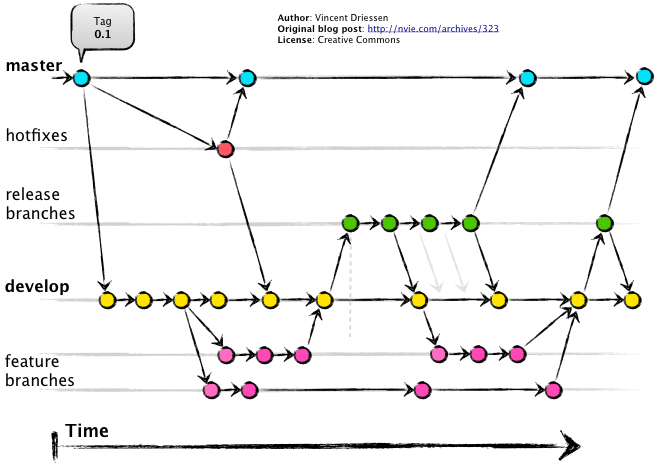
\includegraphics[width=\textwidth]{img/gitflow.png}
\end{center}
\end{frame}
\begin{frame}[label={sec:org027616f}]{Bune practici pentru controlul reviziilor\footnote{\url{https://www.troyhunt.com/10-commandments-of-good-source-control/}}}
\begin{itemize}
\item Dacă nu există în sistemul de control al reviziilor atunci nu există deloc.
\item Fiecare versiune trebuie să fie atomică.
\item Preferați mai multe versiuni mici decât una mare.
\item Descrieți modificările cât mai bine.
\item Nu păstrați istoric pentru fișierele generate la compilare.
\end{itemize}
\end{frame}
\end{document}